% Copyright (C)  2015  Alexander Jankowski, Philipp Hacker.
% Permission is granted to copy, distribute and/or modify this document
% under the terms of the GNU Free Documentation License, Version 1.3
% or any later version published by the Free Software Foundation;
% with no Invariant Sections, no Front-Cover Texts, and no Back-Cover Texts.
% The lincense itself can be found at <https://www.gnu.org/licenses/fdl-1.3>.

\documentclass[numbers=noenddot,a4paper,notitlepage,twoside,BCOR15mm]{scrartcl}
%\documentclass[numbers=noenddot,12pt,a4paper]{scrartcl}

\usepackage{ifoddpage}
\usepackage[infoshow]{tabularx}
\usepackage{fancyhdr}
\usepackage[greek,ngerman]{babel}
\usepackage[T1]{fontenc}
\usepackage[utf8]{inputenc}
\usepackage{libertine}
\usepackage{ziffer}
\usepackage{graphicx}
\usepackage{units}
\usepackage[infoshow]{tabularx}
\usepackage[all]{xy}
\usepackage{amsmath}
\usepackage{amssymb}
\usepackage{wrapfig}
\usepackage{upgreek}
\usepackage{esint}
\usepackage{float}
\usepackage[font=small,labelfont=bf]{caption}
\usepackage{subcaption}
\usepackage{lscape}
\usepackage[backref=page]{hyperref}
\usepackage{cleveref}
\usepackage{csquotes}

\renewcommand{\headrulewidth}{0.1pt}
\renewcommand{\footrulewidth}{0.1pt}
\newcommand{\name}{\text{Philipp Hacker}} %TODO Name des Protokollanten eintragen

\renewcaptionname{ngerman}{\figurename}{Abb. }
\renewcaptionname{ngerman}{\tablename}{Tab.}

\setlength{\parindent}{0pt}

\newcommand{\nummat}[1]{\left[\text{#1}\right]}
\newcommand{\num}[1]{$\left[\text{#1}\right]$}
\newcommand{\degree}{^\circ}
\newcommand{\diff}{\textnormal{d}}
\newcommand{\tenpo}[1]{ 10^{#1}}
\newcommand{\greek}[1]{\greektext#1\latintext}
\newcommand{\ix}[1]{_\text{#1}}
\newcommand{\imag}{\mathbf{i}}
\newcommand{\tilt}[1]{\textit{#1}}
\newcommand{\grad}[1]{\textit{grad}\left(#1\right)}
\newcommand{\divergenz}[1]{\textit{div}\left(#1\right)}
\newcommand{\euler}{\mathnormal{e}}
\newcommand{\fett}[1]{\textbf{#1}}
\newcommand{\einnup}{\hspace{0.2cm}}
\newcommand{\einnum}{\hspace{-0.2cm}}
\newcommand{\zentriert}[1]{\begin{center}#1\end{center}}

\title{Protokoll: Reflektron/\\\tilt{time of flight}-Massespektrometrie} %TODO Name des Versuchs eintragen
\author{Alexander Jankowski, Philipp Hacker}
\date{\today}
\pagestyle{fancy}
\fancyhead[C]{\thepage}
\fancyhead[R]{\name}
\fancyfoot[C]{\thepage}
\fancyhead[L]{Abschnitt \thesection}

\begin{document}
	\maketitle
	\begin{center}
		Betreuer: Marco Rosenbusch \\ %TODO Name des Betreuers eintragen
		Versuchsdatum: 4.11.2015 \\ %TODO Datum des Versuchs eintragen
		\begin{table}[h]
			\centering
			Note: %TODO Gute Note erhalten :)
			\begin{tabularx}{1.5cm}{|X|}
				\hline \\ \\
				\hline
			\end{tabularx}
		\end{table}
	\end{center}
	\vspace*{\fill}
	\tableofcontents
	\vfill
	\newpage
	\section{Motivation}
	
	\newpage
	\section{Physikalische Grundlagen}

		Die in diesem Versuch benutzte Methode der Auflösung und Messung von Massen oder Masse-zu-Ladungs-Verhältnissen ist die der Massenspektrometrie, insbesondere der \tilt{time of flight-Massenspektromertie}.\\
		Dabei werden die zu betrachtenden Teilchen - sein es nun Cluster von mehreren Dutzend Atomen, Moleküle oder deren Monomere bzw. Ionen - in Richtung eines Detektors/Analysators über ein elektrisches Feld beschleunigt. Dabei ist der Strom von, beispielsweise Ionen, möglichst auf eine Bahn fokussiert und quantisiert, sodass hinter der feldfreien Strecke des \tilt{Analysators} die, durch den restlichen Aufbau transmittierten Teilchen nach ihrer Flugzeit im Detektor aufgelöst werden. Die zeitliche Trennung von, notwendigerweise geladenen Probesubstanzen ist Folge der unterschiedlichen Beschleunigungen und damit Geschwindigkeiten aufgrund verschiedener Massen-zu-Landungs-Verhältnissen.\\
		Die Beschleunigung über ein Kondensator-Feld aus \autoref{eq:feld} ergibt die kinetische Energie in \autoref{eq:kinet}. Daraus erkennt man bereits: Teilchen mit gleichen Ladungen aber unterschiedlichen Massen werden verschieden stark beschleunigt, da die kinetische Energie in Abhängigkeit der Potentialdifferenz konstant ist. Vereinfacht man das Problem eines einstufigen \tilt{tof-MS} in einer Dimension - dh. nimmt man an, es gäbe nur eine Stufe $d\ix{1}$ für die Beschleunigung, der Analysator hätte die Länge $d$ und die Ionen würden mit dem Ortsunterschied $\Delta x$ in elektrische Feld mit der thermischen Anfangsgeschwindigkeit aus $qU\ix{th,x}$ eintreten - so ergibt sich die Gesamtflugzeit $t\ix{tof}$ aus der Analysator-Laufzeit $t\ix{d}$ und der Beschleunigungsdauer $t\ix{1}$ in \autoref{eq:tof}.

			\begin{align}
				E\ix{e}=&\frac{U}{d} \label{eq:feld}\\
				E\ix{kin}=qU&=\frac{mv^2}{2} \label{eq:kinet}\\
				\sqrt{\frac{m}{w}}\propto t\ix{tof}=t\ix{1}+t\ix{d}=\sqrt{\frac{m}{q}}\frac{1}{E}&\left[\sqrt{2v\ix{2}}\pm\sqrt{U\ix{th,x}}\right]+\frac{d}{2\sqrt{v\ix{2}}} \label{eq:tof}\\
				v\ix{2}=U\ix{th,x}+&E\left(\frac{d\ix{1}}{2}-\Delta x\right)
			\end{align}

		Das Prinzip der \tilt{tof-MS} greift darauf zurück, das unterschiedlich schnelle Teilchen für eine feldfreie Strecke verschiedene Flugzeiten $t\ix{1}(m\ix{1},q\ix{1}),t\ix{2}(m\ix{2},q\ix{2}),\dots$ benötigen. Das Beispiel in \autoref{eq:tof} kann auf verschiedene Weisen erweitert und verbessert werden. Um den Ortsfokus zu verbessern, dh. den Einfluss von $\Delta x$ und Ablenkungen von der Aufbau-Achse zu minimieren, benutzt man mehrstufige \tilt{tof-MS}und Ionen-Optiken, welche den Teilchenstrom kanalisieren. Wegen der Ortsunschärfe von gleichen Teilchen in der Quelle liegen auch jeweils unterschiedliche Beschleunigungsstrecken vor, weswegen eine 'Verschmierung' der Flugzeit von einzelnen Spezies in Kombination mit der thermischen Verteilung auftritt. Damit dieser Zeitfokus gegeben ist (gleiche Ionen sind zu einer bestimmten Zeit am gleichen Ort), baut man mehrstufige \tilt{tof-MS} mit kleinen und sehr großen Potentialgradienten. Die Auswirkungen von $E\ix{kin,th}$ und $\Delta x$ verschwinden (min. näherungsweise bis zur 2. Ordnung), wobei sich die Gesamtflugdauer um eine Zeit auf der zweiten \dots n-ten Beschleunigungsstrecke erhöht. Insbesondere ist dies der Fall für $d=d\ix{1}$  in der \autoref{eq:tof}.

			\begin{figure}[t]
				\centering
				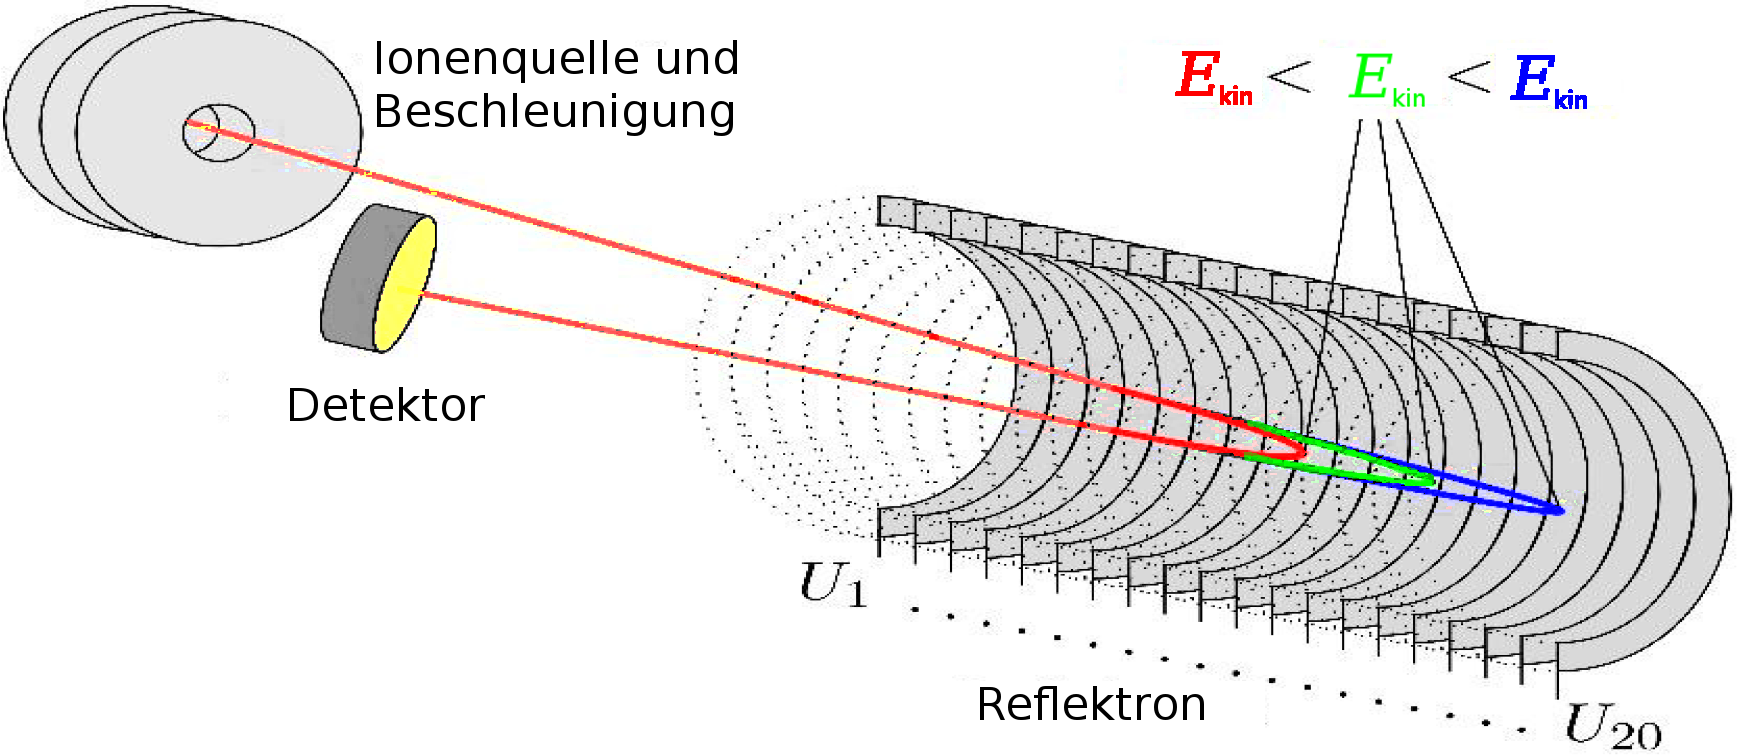
\includegraphics[width=0.8\textwidth]{einspiegel.png}
				\caption{Ein-Spiegel Reflektron mit Ionenquelle, Beschleunigungssektoren und einem Detektor. Hier ist die Abhängigkeit des Eindringens von der kinetischen Energie gezeigt. \cite{EMAUGreifswaldReflektron}}
				\label{img:reflektron1}
			\end{figure}

		Beim sogenannten \tilt{Reflektron} handelt es sich um eine elektrostatische Ionenfalle bzw. Flasche - angelehnt an die elektromagnetische Beschreibung von Elektronen-Bewegungen in Plasmen unter Einfluss eines inhomogenen, gekrümmten Magnetfeldes - welche ein inhomogenes Feld durch viele unterschiedliche Elektroden hintereinander erzeugt. Dieser koaxiale Spiegel reflektiert einfallende Ladungsträger entweder in Richtung des Detektors oder auf einen zweiten, ihm gegenüberliegenden Spiegel (Abhängigkeit von Form des Feldes und der Einfallsrichtung). Teilchen der gleichen Massen-zu-Ladung-Spezies aber mit unterschiedlichen Geschwindigkeiten dringen verschieden weit in das Spiegel-Feld ein. Im speziellen werden sie im Bremsbereich verlangsamt und dann in einem Abschnitt eines flacheren Feldgradienten 'korrigiert' und reflektiert. Dabei dringen zum Beispiel schnellere Teilchen der selben Masse und Ladung tiefer in den Reflektron ein und legen damit mehr Weg zurück, als ihre langsameren Partner. Über die Reflektion werden sie jedoch wiederum stärker und länger beschleunigt, was ihnen ihre Einfallsgeschwindigkeit verleiht. Insgesamt ist bzw. sollte das Reflektron-Feld so geformt sein, dass eben diese, im Impulsraum 'verschmierte' Population einer Probesubstanz an einem fixen Ort innerhalb eines Aufbaus mit 2 Spiegeln zusammenkommt. Unter Umständen ist in Aufbauten mit einem Spiegel ist dieser Ort die Detektoroberfläche.

			\begin{figure}[b]
				\centering
				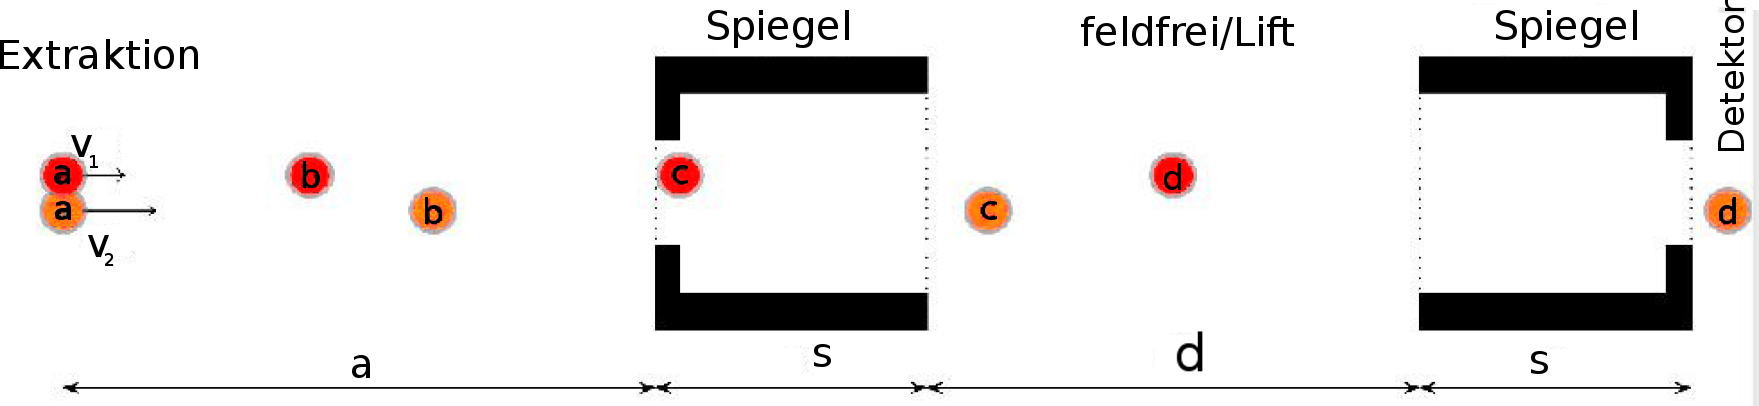
\includegraphics[width=\textwidth]{zweispiegel.png}
				\caption{text}
				\label{img:reflektron2}
			\end{figure}

		Die \autoref{img:reflektron1} und \autoref{img:reflektron2} zeigen den schematischen Verlauf von Ionen aus der Quelle/einer Ionenfalle, in welcher sie gespeichert und selektiert wurden, in einen Ein-Spiegel/Zwei-Spiegel-Reflektron bis auf den Detektor. Zwischen beiden Spiegeln befindet sich eine feldfreie Driftstrecke bzw. ein elektrostatischer 'Lift', welcher den einfallenden/reflektierten Ionen ein neues Bezugspotential verleiht und somit das Eindringen oder Verlassen des Reflektrons ermöglicht. Das Verhältnis von kinetischen Energien, Massen und damit Geschwindigkeiten zweier Ionenspezies, welche im Reflektron verbleiben sollen, ergibt sich mit den Größen $a$, $s$ und $d$ welche \autoref{img:reflektron2} entnommen werden können, in \autoref{eq:speicher}.


		\begin{align}
			\frac{v\ix{1}}{v\ix{2}}=\sqrt{\frac{E\ix{kin,1}m\ix{2}}{E\ix{kin,2}m\ix{1}}}<\frac{a+s+d}{a+s} \label{eq:speicher}
		\end{align}

		Bei einem Multireflexions-Massenspektrometer nutzt man die vielfache Durchquerung des feldfreien Driftbereichs um dicht beeinander liegende Geschwindigkeiten und damit kinetischen Energien deutlich aufzutrennen. Dies spielt eine wichtige Rolle für das Auflösungsvermögen des Experiments, welches als

			\begin{align}
				R=\frac{m}{\Delta m} \label{eq:aufloes}
			\end{align}

		definiert wird. Dabei ist $\Delta m$ unterschiedlich interpretierbar: nach der FWHM-Methode (\tilt{full width at half maximum}) entspricht dieser Wert der Halbwertsbreite des \tilt{gauß'schen} Normalverteilungs-Peaks um die Wahre Masse im Spektrum.

	\newpage
	\section{Durchführung}
	
	\newpage
	\section{Auswertung}
	
	\newpage
	\section{Anhang}

		\bibliography{all.bib}
		\bibliographystyle{unsrt}

\end{document}